% !TEX root = document.tex

\lstdefinestyle{mystyle_regex_comparison}{
language = Python,
otherkeywords = {simpl-rule},
morekeywords = {Choice, Epsilon, Option, Plus, Star, simpl},
keywordstyle = [2]{\color{kw_alt}},
morekeywords = [2]{topdown}
}
\lstdefinestyle{mystyle_small_stratego_listings}{
language = Python,
otherkeywords = {match_a, match_b, match_any_1, match_any_2, do_something_with_A, do_something_with_B, my_strategy, function_1, function_2},
morekeywords = {A, B, C},
keywordstyle = [2]{\color{kw_alt}},
morekeywords = [2]{topdown, all, try, id, fail}
}
\lstdefinestyle{mystyle_map_rule_haskell}{
language = Haskell
}
\lstdefinestyle{mystyle_map_rule_stratego}{
language = Python,
otherkeywords = {r-increment, r-mult, 1, 2},
morekeywords = {E, f},
keywordstyle = [2]{\color{num_color}},
morekeywords = [2]{1, 2},
keywordstyle = [3]{\color{kw_alt}},
morekeywords = [3]{topdown}
}
\lstdefinestyle{mystyle_grafter_example}{
language = Python,
keywordstyle = \color{kw_alt},
keywordstyle = [2]{\color{magenta}},
morekeywords = [2]{increment, multiply, fused_traversal}
}

\chapter{\label{chap:background}Background}
In this chapter, we give background information on the problem of (generic) traversal fusion, and introduce terminology that is useful in working towards a solution for fusion in strategic programming. In addition, we discuss TreeFuser and Grafter: the research on which our solution is based\autocite{SakkaS017, SakkaSN019}. Specifically, we will discuss:

\begin{itemize}
    \item What exactly is a traversal in strategic programming, and what do traversals look like in Stratego?
    \item What exactly does it mean to fuse traversals, and why is it not a trivial problem?
    \item How do TreeFuser and Grafter implement traversal fusion \autocite{SakkaS017, SakkaSN019}?
\end{itemize}

\section{Traversals}
First, we briefly contrast functional programming and strategic programming to show how the separation of rewrite rules and traversals makes strategic programming intuitive when operating on tree-like data structures.

In functional languages, users must explicitly program the order and location in which functions have to be executed to perform a rewrite on input data. This makes the evaluation strategy explicit, but does entangle it with the actual computations. In strategic programming, the evaluation strategy (i.e., traversals) and the computation (i.e., rewrite rules) are separated \autocite{LaemmelVV02}. As an example, consider the comparison of a simplification performed on regular expressions between Haskell and Stratego shown in \autoref{fig:regex-comparison} \autocite{LaemmelVV02}.

\begin{figure}

\begin{subfigure}{\textwidth}
\begin{lstlisting}[language=Haskell, otherkeywords={::, ->, =}, morekeywords={RegExp, Choice, Epsilon, Option, Plus, Star, Seq}]
    simpl :: RegExp -> RegExp
    
    -- rewrite rules
      -- eps | e - > e?
    simpl (Choice Epsilon e) = Option (simpl e)
      -- (e+)? - > e*
    simpl (Option (Plus e)) = Star (simpl e)
    
    -- traversal
    simpl (Star e) = Star (simpl e)
    simpl (Plus e) = Plus (simpl e)
    simpl (Option e) = Option (simpl e)
    simpl (Seq e1 e2) = Seq (simpl e1) (simpl e2)
    simpl (Choice e1 e2) = Choice (simpl e1) (simpl e2)
    simpl e = e
\end{lstlisting}
\subcaption{In Haskell}
\label{fig:regex-comparison-haskell}
\end{subfigure}

\begin{subfigure}{\textwidth}
\begin{lstlisting}[style = mystyle_regex_comparison]
    simpl-rule :
        Choice(Epsilon, e) -> Option(e)
        
    simpl-rule :
        Option(Plus(e)) -> Star(e)
        
    simpl = topdown(simpl-rule)
\end{lstlisting}
\subcaption{In Stratego}
\label{fig:regex-comparison-stratego}
\end{subfigure}

\caption{Comparison of a regular expression simplification program between Haskell and Stratego.}
\label{fig:regex-comparison}
\end{figure}

In the Haskell program, the traversal into every possible constructor has to be explicitly defined. Additionally, the \texttt{simpl} function has to be called in the rewrite rules to make sure the simplification continues to traverse down the AST. In contrast, the rewrite rules and traversal are completely separated in the Stratego program. On top of that, the traversal is also defined generically in the Stratego program: \texttt{topdown} works for all constructors.

\subsection{Definition}
We now define exactly what we mean by a traversal, or a strategy in Stratego. There is a subtle difference between the terms traversal and strategy: a traversal is a specific way to iterate over a data structure. A strategy is the way to define a traversal on a data structure in a strategic programming language. For the purposes of traversal fusion, talking about the traversal or the strategy that defines it usually does not cause confusion. For example, Stratego's \texttt{topdown} strategy defines a top-down traversal. The algorithm we have developed fuses traversals, but these traversals are \textit{represented} as strategies.

Strategies do have some specific properties that are important to mention. Strategies are \autocite{LaemmelVV02}: 

\begin{itemize}
    \item \textbf{Generic} - applicable to data of any shape;
    \item \textbf{Specific} - provide access to data structures on which they operate;
    \item \textbf{Partial} - may fail;
    \item \textbf{First-class} - they can be named and passed as arguments,
\end{itemize}

\noindent and enable

\begin{itemize}
    \item \textbf{Traversal} - generic traversal into subcomponents of data structures;
    \item \textbf{Control} - can model control over the application of computations (i.e. the application of rewrite rules).
\end{itemize}

These properties define the basic building blocks that can be used to define traversals in any strategic language.

\subsection{Stratego Traversals}
There are six basic strategy building blocks that arise from the aforementioned properties for any strategic programming language \autocite{LaemmelVV02}. These are also exactly the building blocks available in Stratego. Because these building blocks are the essence of the way to define traversals in Stratego, they will be used extensively in this thesis. We will list them here, and show how they might be used to define some basic strategies, or traversals. The six building blocks are:

\begin{itemize}
    \item Identity (\texttt{id}) - always succeeds and does nothing when applied to any term
    \item Failure (\texttt{fail}) - always fails when applied to any term
    \item Sequence (\texttt{\_;\_}) - first applies its left-hand argument, then applies its right-hand argument to a term
    \item Conditional (\texttt{\_<\_;\_}) - Attempts to apply its first argument. If this succeeds, it then applies its second argument to the result. Otherwise, it applies its third argument to the original term.
    \item All (\texttt{all(\_)}) - Applies its argument to all (direct) children of the current term. Fails if any application fails.
    \item One (\texttt{one(\_)}) - Attempts to apply its argument to all (direct) children of the current term, but stops upon the first successful application. Fails if all applications fail.
\end{itemize}

In addition to having these building blocks available, it is also legal to use recursive definitions in Stratego. This enables the definition of several important strategies, such as \texttt{topdown}:

\begin{lstlisting}[style = mystyle_small_stratego_listings]
    topdown(s) = s; all(topdown(s))
\end{lstlisting}

\noindent The \texttt{topdown} strategy takes one argument, \texttt{s}. When applying the \texttt{topdown} strategy to a node, it uses the sequence operator (\texttt{;}) to first apply \texttt{s} to that node. Then, it uses \texttt{all} to apply \textit{itself} to all children of the node. Indeed, this strategy exactly defines a top-down traversal.

Another useful strategy is \texttt{try}. This strategy attempts to apply its argument. However, if this fails, the \texttt{try} strategy itself does not fail:

\begin{lstlisting}[style = mystyle_small_stratego_listings]
    try(s) = s < id + id
\end{lstlisting}

\subsection{Additional Stratego Syntax}
\label{sec:additional-stratego-syntax}
We discuss two additional Stratego syntax features that are used in this thesis: matches and congruences.

First, matches allow for matching on a term inside a strategy. We use this to dynamically check the constructor of a node in our fused traversal functions, in combination with the conditional operator. The match operator is a question mark \texttt{?}. It succeeds if the match succeeds on the current node, and it fails if the match fails. For example, consider two constructors \texttt{A} and \texttt{B}, both with one subterm of type \texttt{Int}. The current node is \texttt{A(1)}. Then,

\begin{lstlisting}[style = mystyle_small_stratego_listings]
    match_a = ?A(_)         [succeeds]
    match_b = ?B(_)         [fails]
    match_any_1 = ?_(_)     [succeeds]
    match_any_2 = ?_(_, _)  [fails]
\end{lstlisting}

In combination with the conditional operator, we could construct a match chain like so:

\begin{lstlisting}[style = mystyle_small_stratego_listings]
    ?A(_) < do_something_with_A + ?B(_) < do_something_with_B + fail
\end{lstlisting}

Another important syntax feature of Stratego is the congruence operator, which applies strategies to subterms of a constructor. This operator allows for, among other things, the application of different functions to different children of a node. This is necessary to construct our fused traversal functions. The congruence operator looks like a constructor application, but we provide strategies as subterms. For example, the following applies the \texttt{id} strategy to the first child of a constructor \texttt{C}, some \texttt{function\_1} to its second child, and some \texttt{function\_2} to the last:

\begin{lstlisting}[style = mystyle_small_stratego_listings]
    my_strategy = C(id, function_1, function_2)
\end{lstlisting}

\section{Traversal Fusion}
Having defined what we mean by traversals and strategies in strategic programming, we can now look at the problem of traversal fusion. Traversal fusion is the process of taking multiple traversals and altering them in such a way that program results are maintained, but the data structure is traversed in a different way. The aim is to reduce the number of total unique visits to nodes in the data structure. Generic traversal fusion refers to the idea of doing this for generic strategies.

As an example of how fusion might work, consider a concept from functional programming that seems similar. If a function \texttt{f} is mapped over a data structure (say, a list), and then a different function \texttt{g} is mapped over the resulting list, that is the same as mapping the composition of \texttt{f} and \texttt{g} over the original list just once. So, we have that:

\begin{lstlisting}[language=Haskell, otherkeywords={=, .}]
    map f; map g = map (g . f)
\end{lstlisting}

\noindent For example, consider mapping the function \texttt{(+ 1)} over a list of integers, and then the function \texttt{(* 2)} as shown in \autoref{fig:map-rule}. Without changing the functions themselves, a traversal of the list was created that visits every element only once, but achieves the same result as the sequence of two traversals (that, in total, visit every node in the list twice).

\begin{figure}
\begin{lstlisting}[style = mystyle_map_rule_haskell]
    [1, 2, 3, 4, 5]
      -- map (+ 1)
    [2, 3, 4, 5, 6]
      -- map (* 2)
    [4, 6, 8, 10, 12]

    [1, 2, 3, 4, 5]
      -- map ((* 2) . (+ 1))
    [4, 6, 8, 10, 12]
\end{lstlisting}
\caption{An example of the map rule.}
\label{fig:map-rule}
\end{figure}

Consider how this might apply to strategies operating on trees (for this example, trees in which nodes have just one child). Define a rewrite rule that increments every node by one in such a tree. Similarly, define a rewrite rule that multiplies the values by two. Applying these rules top-down would lead to the same situation as the \texttt{map} in functional programming, as shown in \autoref{fig:map-rule-analogy}.

\begin{figure}
\begin{lstlisting}[style = mystyle_map_rule_stratego]
    r-increment:
        E(v, c) -> E(v + 1, c)

    r-mult:
        E(v, c) -> E(v * 2, c)

    f = topdown(r-increment); topdown(r-mult)
\end{lstlisting}
\caption{A situation analogous to the map rule example in Stratego.}
\label{fig:map-rule-analogy}
\end{figure}

These top-down traversals could be fused together like the \texttt{map}: \texttt{topdown(r-increment; r-mult)} achieves the same end result, while only visiting every node of the tree once.

%The goal of traversal fusion is not to necessarily optimize the actual algorithm being computed on the data structure. We only aim to compute it in a different way that saves as much traversal overhead as possible: doing as much work as we can in as few unique node visits as possible.%

Unfortunately, it is not always easy to determine whether a traversal fusion is legal. Indeed, the example of fusing the two top-down traversals together happens to be legal in that specific example, but it is not always legal. So, unlike the \texttt{map} rule in functional programming, \texttt{topdown(r1); topdown(r2)} is \textit{not} always equivalent to \texttt{topdown(r1; r2)}! As a counter-example, simply consider again the copy-up example shown in \autoref{fig:twotd-counterexample} in \autoref{chap:introduction}.

So \texttt{topdown(r1); topdown(r2) = topdown(r1; r2)} is sometimes true, and sometimes false, depending on the specific rewrite rules. However, there are some fusions that are always legal. One example is \texttt{downup}, defined in the Stratego standard library. When performing a top-down traversal followed by a bottom-up traversal, \texttt{downup} can save some overhead by not having to go down the tree again after the top-down traversal. This is always legal.

However, these fusions that are always legal seem to be rare. To achieve fusion in most cases, it is necessary to look at the exact rewrite rules and traversals performed by a program, and determine for that specific program whether fusion can be performed. Research has been done on using dependency analysis on programs for this purpose \cite{SakkaS017, SakkaSN019}, and this is also the approach we use to achieve traversal fusion in strategic programming. This will be discussed in more detail below.

\section{Towards a Solution}
\label{sec:towards-a-solution}
TreeFuser and Grafter are two related algorithms that can perform traversal fusion in a C-like imperative language through the use of dependency analysis \autocite{SakkaS017, SakkaSN019}. This means that statements are analyzed and placed in a dependence graph in which edges represent dependency relations. For example, a write followed by a read on the same location would introduce a dependency edge as it would not be legal to perform the read before the write.

There are important differences between TreeFuser and Grafter. In essence, Grafter is an extension of TreeFuser that supports more language features, and can find more opportunities for fusion. The differences will be explained in more detail at the end of this section.

Because traversals are represented as recursive functions in this C-like language, the recursive calls are also statements and also placed in the dependence graph. This makes it possible to re-order and even merge these calls, as long as that would not create a dependency violation (i.e., a cycle in the dependence graph). We will show that if calls can be merged, a legal opportunity for traversal fusion has been found.

The four main steps of the TreeFuser algorithm are:
\begin{enumerate}
    \item Performing a dependency analysis;
    \item Building a dependence graph;
    \item Finding fusion opportunities in the dependence graph;
    \item Synthesizing a program with fused traversals where possible.
\end{enumerate}

\autoref{fig:treefuser-example} shows these steps on a similar program to the map rule example program from \autoref{fig:map-rule} and \autoref{fig:map-rule-analogy}.

\begin{figure}

\begin{subfigure}{\textwidth}
\begin{lstlisting}[style = mystyle_grafter_example]
    increment(n)
      n.v = n.v + 1     [s1]
      increment(n.l)    [c1]
      increment(n.r)    [c2]

    multiply(n)
      n.v = n.v * 2     [s2]
      multiply(n.l)     [c3]
      multiply(n.r)     [c4]
\end{lstlisting}
\subcaption{Increment and multiply top-down functions}
\label{fig:treefuser-example-1}
\end{subfigure}

\begin{subfigure}{\textwidth}
\begin{lstlisting}
    s1 (line 2) :
      R : n.v
      W : n.v
    c1 (line 3) :
      R : n.l(.l|.r)*.v
      W : n.l(.l|.r)*.v
    c2 (line 4) :
      R : n.r(.l|.r)*.v
      W : n.r(.l|.r)*.v

    s2 (line 7) :
      R : n.v
      W : n.v
    c3 (line 8) :
      R : n.l(.l|.r)*.v
      W : n.l(.l|.r)*.v
    c4 (line 9) :
      R : n.r(.l|.r)*.v
      W : n.r(.l|.r)*.v
\end{lstlisting}
\subcaption{Dependency analysis results}
\label{fig:treefuser-example-2}
\end{subfigure}

\begin{subfigure}{0.5\textwidth}
\centering
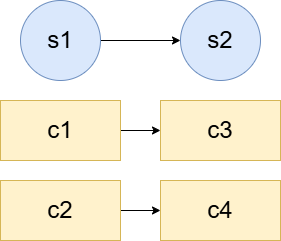
\includegraphics[width=5cm]{./img/treefuser-example-dgraph.png}
\subcaption{Dependence graph before fusion}
\label{fig:treefuser-example-3}
\end{subfigure}%
\begin{subfigure}{0.5\textwidth}
\centering
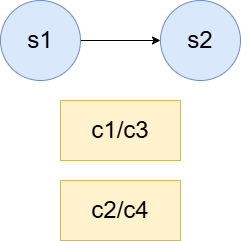
\includegraphics[width=4.3cm]{./img/treefuser-example-dgraph2.png}
\subcaption{Dependence graph after fusion}
\label{fig:treefuser-example-4}
\end{subfigure}

\begin{subfigure}{\textwidth}
\begin{lstlisting}[style = mystyle_grafter_example]
    fused_traversal(n, do_1, do_2)
      if do_1
        n.v = n.v + 1                   [s1]
      if do_2
        n.v = n.v * 2                   [s2]
      fused_traversal(n.l, do_1, do_2)  [c1/c3]
      fused_traversal(n.r, do_1, do_2)  [c2/c4]
\end{lstlisting}
\subcaption{Example resulting fused code}
\label{fig:treefuser-example-5}
\end{subfigure}
\caption{An example of the TreeFuser algorithm.}
\label{fig:treefuser-example}
\end{figure}

In \autoref{fig:treefuser-example-1}, the two functions are defined. Each function consists of three statements: the transformations (on lines 2 and 7, respectively), and the recursive calls for the traversals (lines 3 and 4, and lines 8 and 9). We will call the statements from the \texttt{increment} function \texttt{s1}, \texttt{c1}, and \texttt{c2}. The statements from the \texttt{multiply} function will be called \texttt{s2}, \texttt{c3}, and \texttt{c4}. Both \texttt{s1} and \texttt{s2} (the transformations) perform a read and write on \texttt{n.v}. The recursive calls traverse down into either \texttt{n.l} or \texttt{n.r}, and then execute the function they called on that node. That means they perform a read and write on either \texttt{n.l.v} or \texttt{n.r.v}, but also recursively continue to traverse down into the children of either \texttt{n.l} or \texttt{n.r}. Effectively, this constructs a regular expression that describes the reads and writes of these calls, as shown in \autoref{fig:treefuser-example-2}.

A dependence graph can be constructed based on the results of the dependency analysis by checking where two statements access the same location, with at least one of the statements being a write. For any such access intersection, an edge is added in the dependence graph between the two statements to maintain their relative ordering. The result of this is shown in \autoref{fig:treefuser-example-3}. In this case, there are only three edges.

The algorithm then attempts to merge nodes in the dependence graph, which represents traversal fusion. It is only legal to merge call nodes. These call nodes also have to, logically, traverse down into the same child to be able to be fused. This means a fusion of \texttt{c1} with \texttt{c3} is possible in this example, as well as a fusion of \texttt{c2} with \texttt{c4}. The resulting dependence graph is shown in \autoref{fig:treefuser-example-4}. Because this fusion has not resulted in any cycles in the dependence graph, it is also a legal fusion.

We will not discuss the final step (the synthesis of the fused traversal code) in detail here, but possible fused code that could be generated for this example has been included in \autoref{fig:treefuser-example-5}. In essence, a topological order for all statements is extracted from the dependence graph after fusion, and a function is then built from statements in that order. In this case, this does indeed result in a fused function that performs fewer total node visits than the unfused version, which might already be inferred from the fact that there are only two call nodes remaining instead of four.

An important benefit of both the TreeFuser and Grafter algorithms is that they support the concept of partial fusion, enabling many more fusion opportunities than algorithms that look only at opportunities for full fusion. Consider, for example, a scenario in which \texttt{c1} and \texttt{c3} could be fused in the previous example, but \texttt{c2} and \texttt{c4} could not. That implies that the traversals can be merged on the left children of a node, but not on the right children. This leads to a somewhat unusual fused traversal, but one that does perform fewer total node visits.

The most important difference between TreeFuser and Grafter, then, is that TreeFuser assumes trees are homogeneous (consist of only a single constructor). Grafter performs a more complex analysis that allows heterogeneous trees (multiple different constructors) to be analyzed, and also enables type-specific partial fusion. That means fusion cannot only be performed on some children but not on others, but also on some constructors but not on others. 

In addition, both TreeFuser and Grafter are formally proven to be sound, and thus provide a solid basis for a strategic programming traversal fusion algorithm. There are, however, also important differences between imperative and strategic programming and limitations of both algorithms that need to be addressed to achieve traversal fusion in strategic programming. The most important of these are:

\begin{itemize}
    \item In strategic programming, the transformations and traversals are explicitly separated, instead of incorporated into a single function that can be analyzed
    \item In strategic programming, traversal functions are not normally represented as functions that make recursive calls on individual children
    \item In strategic programming, transformations are not represented as statements, but rather as rewrite rules that make their reads and writes less explicit
    \item Neither algorithm supports conditionally made recursive calls, which are much more common in strategic programming
    \item Code synthesis must logically result in a strategic program, not an imperative one
    \item Strategies are definitionally generic, making support for heterogeneous trees unavoidable, and complicating most steps of the algorithm
\end{itemize}

In the next chapter, we will demonstrate a solution for traversal fusion in strategic programming based on a combination of both of these algorithms, and that incorporates new methods to work around the issues outlined above.

%And the fact that it's not really fusion of traversals but of recursive calls in a 'traversing function'... A method inspired by this for strategic programming, could that work?%

%If it does work, can we extract features of the rules for which it works, to have a way of sort of saying 'if your rules obey X, Y, Z constraints, you can fuse certain traversals generically like so' without necessarily specifying the rules completely? E.g. sequential topdown for rules that only look at direct children. Provable through \autocite{SakkaS017, SakkaSN019} method?%